\documentclass[10pt,a4paper]{article}
\usepackage[utf8]{inputenc}
\usepackage[english]{babel}
\usepackage[square, numbers, sort&compress]{natbib}
\usepackage{graphicx}
\usepackage{float}
\usepackage{amsmath}
\usepackage{amsfonts}
\usepackage{amssymb}
%\usepackage{media9}
\usepackage{color}
\usepackage{fancyhdr}
\usepackage{lastpage}	
\usepackage{parskip}
\usepackage[scaled]{helvet}
\usepackage{blindtext}
\usepackage{sectsty}
\usepackage{multicol}
\usepackage{enumitem}
%\usepackage[svgnames]{xcolor}
\usepackage[labelfont={color=LibrelloColor,bf}, labelsep=period]{caption}
\renewcommand*{\familydefault}{\sfdefault}
\usepackage[left=1.75cm,right=1.75cm,top=1.75cm,bottom=3.75cm]{geometry}
\usepackage{titlesec}
\usepackage{svg}
\usepackage{flushend}
\PassOptionsToPackage{normalem}{ulem}
\usepackage{ulem}
	\providecolor{added}{rgb}{0,0,1}
	\providecolor{deleted}{rgb}{1,0,0}
	%% Change tracking with ulem
	\newcommand{\added}[1]{{\color{added}{}#1}}
	\newcommand{\deleted}[1]{{\color{deleted}\sout{#1}}}
\usepackage{setspace}
\usepackage[hyphens]{url}

% Green - CiS, OF
\definecolor{LibrelloColor}{RGB}{0,85,0}
% Red - JoHS
%\definecolor{LibrelloColor}{RGB}{128,0,0}



\usepackage[hidelinks, urlcolor=LibrelloColor]{hyperref}
\urlstyle{same}
\raggedcolumns
\flushcolumns
\usepackage{etoolbox}
%\usepackage{caption}
\usepackage{supertabular}
\usepackage{booktabs}
\usepackage{microtype}
\usepackage{threeparttable}
\usepackage{doi}
\usepackage{balance}
\usepackage{enumitem}
\usepackage{eurosym}
\usepackage{epstopdf}

\usepackage[color=yellow,icon=Comment,hoffset=-10mm, author=Librello Editorial's Office]{pdfcomment}

\titleformat{\section}
{\color{LibrelloColor}\normalfont\bfseries\filright}
{\color{LibrelloColor}\thesection.}{0.5em}{}

\titleformat{\subsection}
{\color{LibrelloColor}\normalfont\itshape\filright}
{\color{LibrelloColor}\thesubsection.}{0.5em}{}

\titleformat{\subsubsection}
{\color{LibrelloColor}\normalfont\itshape\filright}
{\color{LibrelloColor}\thesubsubsection.}{0.5em}{}

\usepackage{array} %criando coluna de largura fixa alinhada a esquerda
\newcolumntype{L}[1]{>{\raggedright\let\newline\\\arraybackslash\hspace{0pt}}p{#1}}
%criando coluna de largura fixa alinhada a direita
\newcolumntype{R}[1]{>{\raggedleft\let\newline\\\arraybackslash\hspace{0pt}}p{#1}}
\renewcommand{\arraystretch}{1.3}
\titlespacing\section{0pt}{12pt}{12pt}
\titlespacing\subsection{0pt}{12pt}{12pt}
\titlespacing\subsection{0pt}{12pt}{12pt}	
\renewcommand*{\refname}{References and Notes}

\fancypagestyle{document}{
	\renewcommand{\footrulewidth}{0pt}
	\renewcommand{\headrulewidth}{0pt}
	\renewcommand{\footrulewidth}{0pt}
	\renewcommand{\headrulewidth}{0pt}
	\renewcommand{\footskip}{40pt}
	\cfoot{\normalfont\thepage}
	\rhead{}\lhead{}
}

\fancypagestyle{firstpage}{
	\renewcommand{\footrulewidth}{0pt}
	\renewcommand{\headrulewidth}{0pt}
	\renewcommand{\footrulewidth}{0pt}
	\renewcommand{\headrulewidth}{0pt}
	\renewcommand{\footskip}{70pt}
	%CiS
	\lhead{Challenges in Sustainability $\mid$ 2017 $\mid$ Volume 5 $\mid$ Issue 1 $\mid$ Pages \thepage--\pageref{LastPage} \\DOI: 10.12924/cis2017.05010007\\
	ISSN: 2297--6477}
	\rhead{\includegraphics[height=0.59in]{CiS.eps}}
	%JoHS
%	\lhead{Journal of Human Security $\mid$ 2016 $\mid$ Volume 12 $\mid$ Issue 1 $\mid$ Pages \thepage--\pageref{LastPage} \\DOI: 10.12924/johs2016.12010112\\
%	ISSN: 1835--3800}
%	\rhead{\includegraphics[height=0.59in]{JoHS.eps}}
	%OF
%	\lhead{Organic Farming $\mid$ 2016 $\mid$ Volume 2 $\mid$ Issue 1 $\mid$ Pages \thepage--\pageref{LastPage} \\DOI: 10.12924/of2016.02010023\\
%	ISSN: 2297--6485}
%	\rhead{\includegraphics[height=0.59in]{OF.eps}}	
	\lfoot{\footnotesize © 2017 by the authors; licensee Librello, Switzerland. This open access article was published\\ under a Creative Commons Attribution License (\url{http://creativecommons.org/licenses/by/4.0/}).}
	\cfoot{}
	\rfoot{\vspace*{-24pt}\includegraphics[height=0.49in]{librello.eps}}

}

\makeatletter
\def\NAT@def@citea{\def\@citea{\NAT@separator}}
\makeatother

\begin{document}
\flushcolumns
\raggedcolumns



\pagestyle{document}
\thispagestyle{firstpage}


\vspace*{70pt}

\setlength{\parindent}{0cm}
\textit{Research Article}
%\textit{Review}
\vspace*{-12pt}

\begin{center}
\line(1,0){500}
\end{center}

\vspace*{12pt}
\begin{flushleft}
\begin{LARGE}
\textbf{{\color{LibrelloColor} Alternative Perspectives on Sustainability: Indigenous Knowledge and Methodologies}}\\
\end{LARGE}

\vspace*{12pt}

Meg Parsons$^{1,}$*, Johanna Nalau$^{2,3}$* and Karen Fisher$^{1}$

\vspace*{6pt}

$^1$ School of Environment, University of Auckland, Auckland, New Zealand. E-Mail: k.fisher@auckland.ac.nz (KF)\\
$^2$ Griffith Climate Change Response Program (GCCRP), Griffith University, Nathan, Australia\\
$^3$ Griffith Institute for Tourism (GIFT), Griffith University, Nathan, Australia\\


\vspace*{6pt}

* \textls[-15]{Corresponding author: E-Mail: meg.parsons@auckland.ac.nz (MP), j.nalau@griffith.edu.au (JN) ; Tel.: +61 755527257 (JN)}

\vspace*{6pt}

Submitted: 20 April 2016 $\mid$ In revised form: 7 October 2016 $\mid$ Accepted: 6 December 2016 $\mid$\\
Published: 22 February 2017
\end{flushleft}
\setcounter{page}{7}


\vspace*{-18pt}
\begin{center}
\line(1,0){500}
\end{center}

\vspace*{12pt}
%\vspace{\baselineskip}

\begingroup\leftskip= 1cm\rightskip 1cm  

\textbf{{\color{LibrelloColor}Abstract:}} Indigenous knowledge (IK) is now recognized as being critical to the development of effective, equitable and meaningful strategies to address socio-ecological crises. However efforts to integrate IK and Western science frequently encounter difficulties due to different systems of knowledge production and underlying worldviews. New approaches are needed so that sustainability can progress on the terms that matter the most for the people involved. In this paper we discuss a case study from Aotearoa New Zealand where an indigenous community is in the process of renegotiating and enacting new indigenous-led approaches to address coupled socio-ecological crises. We reflect on novel methodological approaches that highlight the ways in which projects/knowledge are co-produced by a multiplicity of human and non-human actors. To this end we draw on conceptualizations of environmental ethics offered by indigenous scholars and propose alternative bodies of thought, methods, and practices that can support the wider sustainability agenda.

\textbf{{\color{LibrelloColor}Keywords:}} Aotearoa New Zealand; climate adaptation; colonialism; culture; Indigenous Knowledge; sustainability science
\par\endgroup
 
\setlength{\parindent}{0.5cm}
\setlength{\parskip}{0cm}
\setlength{\bibsep}{0cm}

\vspace*{10mm}
%\vspace*{20mm}

\begin{multicols}{2}

\section{Introduction}
\noindent \textls[15]{Globally, researchers and policy makers are increasingly recognizing the importance of Indigenous Knowledge (IK) in the development and implementation of policies and management approaches \citep{r01} . The recent Intergovernmental Panel on Climate Change's (IPCC) Fifth Assessment Report signals this importance of IK as a building block of human security in stating that there is a high likelihood and robust evidence to demonstrate that ``indigenous, local and traditional forms of knowledge are a major resource for adapting to climate change'' (\citep{r02}, p. 758). The integration of such bottom-up place-based knowledge with science is hoped to promote more robust approaches in increasing community resilience, adaptation, sustainability, and disaster preparedness \citep{r03}. This is based on the premise that the integration of scientific and other knowledge systems can ``lead to a more effective interface between science, policy and society” (\citep{r04}, p. 4). We argue that the transdisciplinary nature of sustainability science has the potential to examine the world through a more holistic approach, something that is often associated with indigenous groups' way of viewing the world. In this paper, our main aim is to discuss the range of challenges regarding integration, the ways IK is currently understood and researched, and the need for recognition of historical ideologies and processes, particularly in relation to matters of equity, accountability and fairness in indigenous- related research.}

\textls[30]{The interest in IK has partly emerged through decades of `failed' development and the recognition that participatory, locally-led and locally-informed processes are more attuned to indigenous groups' priorities and aspirations  \citep{r01}. Attempts to integrate IK with Western scientific knowledge often struggle, however, due to the problematic treatment of IK by scholars. The dominant framing of IK is as a complementary source of knowledge to (Western) science, which can be used to augment empirical data on local environmental conditions including the status of biodiversity \citep{r05}, impacts of climate variability and change \citep{r06, r07}, and frequency of hazards \citep{r08, r09, r10}. This is problematic because it positions scientific knowledge as objective, rational, and universal and IK as highly situated, specific, embedded, and subjective. Thus scholars criticize Indigenous Knowledge-holders for having ``inaccurate and poor conception\ldots of past ecosystems and the changes undergone in their surrounding environment'' (\citep{r05}, p. 279), without acknowledging, for instance, the impacts of colonization and globalization on IK traditions. There is also little appreciation or questioning of the knowledge base/roots where Western science and colonialism originated from, with their conceptual roots in European local histories that have became globally applied \citep{r11}.}

Instead of direct comparisons with Western scientific knowledge, IK systems should be viewed as different but nevertheless equally valid ways of understanding the world \citep{r12}. IK systems can be defined as ``the combination of knowledge systems encompassing technology, social, economic, and philosophical learning, or education, legal and governance systems'' (\citep{r13}, p. 8). Indigenous approaches therefore use, for example, reciprocity as part of the process in responding to social problems and perceive themselves as ``respectful partners in genealogical relationships of interconnected humans, non-human beings, entities and collectives who have reciprocal responsibilities to one another'' (\citep{r14}, p. 25; Figure \ref{Fig01}). Greater appreciation and consideration of IK is crucial if sustainability science is to encapsulate and build upon people’s values and worldviews in a meaningful manner \citep{r02, r15, r16}.


\end{multicols}

\vspace{2\baselineskip}


\noindent
\begin{minipage}{\columnwidth}
\centering
\resizebox{\columnwidth}{!}
{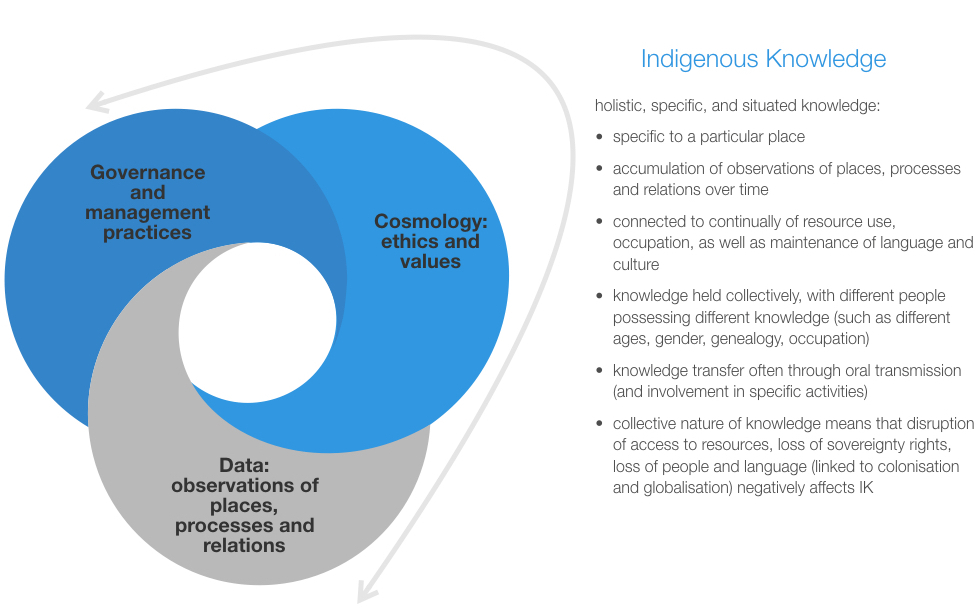
\includegraphics[width=\textwidth]{Fig01.jpeg}}
\captionof{figure}{The different dimensions of Indigenous Knowledge and its basis. \label{Fig01}}
\end{minipage}

\clearpage

\begin{multicols}{2}

While it is outside the scope of this paper to provide a review of the definitional differences, sustainability is broadly defined by scholars in terms of the themes of interconnection of the social, economic, and environmental domains and intergenerational resource usage and requirements. Cutter (\citep{r17}, p. 73) defines sustainability as ``the potential to maintain the long term well-being of communities based on social, economic, and environmental requirements of present and future generations'' (\citep{r17}, p. 73). One of the challenges for sustainability science is to diversify the meaning of sustainability and well-being, which so far have been reliant on measures such as GDP. The incorporation of indigenous conceptualizations of well-being and sustainability, and their inclusion as driving values in policy and research, potentially offer a more inclusive platform for an enriched conversation as to what the goals and outcomes should be and why. This is crucial given that issues of equity and fairness are at the core of any discussion on sustainability \citep{r18}. Moreover, an increase in `reflexive science' \citep{r19, r20} is helpful for enhancing the validity of, and accountability in, sustainability science. Reflexive approaches which call for a greater recognition of both of our personal norms and values and those at work in processes where knowledge is generated and assessed could offer an avenue for a broader acknowledgement of indigenous perspectives and ways of being.

The paper is organized in the following manner: the next section examines the role of IK in sustainability science and the range of issues that arise in conducting indigenous-related research. The third section presents the case study of indigenous sustainability research from Aotearoa New Zealand where a new innovative knowledge integration methodology is used to provide a more inclusive and holistic approach to the notion of sustainability. This example is used to demonstrate the underlying different worldviews that IK holders and scientists often have and to highlight the necessity of considering the differences and similarities of different types of knowledges in knowledge production processes. This, we argue, does not mean only considering IK but finding innovative ways to understand and consider the multiplicity of meanings that exist in each context and influence what `sustainability' can and should look like. The last section summarizes the main points of the paper and also provides some suggestions how to move forward in this area of research.



\section{Synthesis of IK Methodologies and Sustainability}
\noindent Sustainability science has been critiqued for not giving indigenous issues and knowledge a prominent place in its investigations \citep{r21}. For example, the proposed Sustainability Science research agenda \citep{r22} that sought to define the domain of sustainability science makes no mention of indigenous groups or differential vulnerabilities across particular groups in society. While many of the proposed research themes can certainly be applied to indigenous sustainability research, the agenda treats `society', to some extent, as a somewhat uniform collective, with agreed processes of knowledge production. Yet, recently some sustainability scientists are starting to recognize IK as an integral part of sustainability science and draw attention to the ways IK can contribute to the research agenda \citep{r21, r14}.

\textls[10]{It is important to recognize the colonial histories and origins of many of the social sciences, and the ways in which research was used to justify colonial rule over indigenous and non-white (non- indigenous) populations \citep{r23}.  In particular geographical knowledge about environment, race, and health were intricately bound up with the emergent systems of governance in colonial societies \citep{r23}. Theories of environmental determinism sought to explain indigenous populations' `primitivism' as a consequence of environmental constraints and racial deficits, which in turn informed colonial policies that sought to exclude or marginalize indigenous and other non-white (non-indigenous) populations \citep{r24, r25}.}

Coombes et al. (\citep{r26}, p. 846) argue that place-based ethnographies, a popular approach in global environmental research, all too frequently \ldots frame Indigenous peoples as eco-friendly denizens of particular localities\ldots which seek to lock Indigenous peoples into pre-modern development, perpetuate gender bias, or invalidate national-scale activism''. Cameron \citep{r27}, Watson and Huntington \citep{r28}, and Parsons \citep{r25} critique in turn how indigenous experiences in a diversity of contexts (the North America Arctic, Australia) are narrated in the climate change scholarship as either passive victims or heroic resistance to external forces, which subtly works towards reinforcing a disabling social pathology \citep{r29}.

\textls[-20]{One of the most frequent objections to research pertains to intellectual property rights, and the appropriation of IK by researchers and the use of this knowledge for economic purposes (such as
the commercialization and copyrighting of IK about biological agents).Akom \citep{r30} and Coombes et al. \citep{r26} draw on Freie's ideas of liberatory praxis as a way to address indigenous peoples’ objections to research through a deliberate shift away from neocolonial representations of the indigenous Other towards indigenous social science research centered on advocacy, activism and collective problem-solving. In an indigenous context, how knowledge is created and transferred, and the kinds of social relationships that are built, are an important part of the `engagement' that determines the extent to which knowledge is considered useful for communities. Participation and dialogue should therefore be at the heart of this engagement to ensure the research and policy initiatives address and fit within the communities' priorities \citep{r31}.}

Understanding power relations and rights to knowledge dissemination is equally important. A research project examining indigenous weather forecasts in Vanuatu considered these dimensions and enabled the indigenous participants to first agree on the kind of information that could be reported for the general public and was not considered sacred or owned by particular bloodline or role in the community \citep{r32}. Indeed this shift, we suggest, should be at the heart of emergent Indigenous co-design research projects that aim to understand the indigenous socio- political transformations to more sustainable futures. Next, we present a case study that looks at how Indigenous values and perceptions can provide the basis for a more inclusive multi-value management approach and one of the bases for sustainability research and policy formulation.

\section{Case Study: Rethinking the Future of Freshwater Systems in Aotearoa New Zealand}
\noindent InAotearoa New Zealand, freshwater systems are affected by persistent degradation due to human activities. Some of the most immediate problems include nutrient contamination, heavy metals, flooding, biodiversity loss, invasive species, and over extraction. These problems present ongoing threats to the health and well-being of both ecological and human communities. Researchers at the University of Auckland are undertaking a transdisciplinary research project that investigates attempts to accommodate m\={a}tauranga M\={a}ori (M\={a}ori IK) and scientific knowledge in river co- governance and co-management. The three-year project (2016--2018) investigates the ways in which Ng\={a}ti Maniapoto (a M\={a}ori iwi or tribe in the central North Island) are asserting m\={a}tauranga and kaitiakitanga (M\={a}ori stewardship according to iwi aspirations and practices) in relation to the co-governance and co-management of the Waip\={a} River.

The Waip\={a} River is the major tributary of the Waikato River, New Zealand's longest river, and has been identified as one of the most degraded freshwater systems in Aotearoa New Zealand \citep{r33, r34}. The Waip\={a} River and its tributaries flow through environments that have been radically changed by human activities over the last 180 years. The consequences of radical environmental changes within the river catchment now present challenges for local communities and institutions (including local iwi). Co-governance and co-management of the Waip\={a} River are formalized through legislation passed in 2012 (Nga wai o Maniapoto (Waip\={a} River) Act 2012) following the settlement of a Treaty of Waitangi claim. The Treaty settlement was enabled by right to redress for grievances under the Treaty of Waitangi, which was signed by representatives of the British Crown and M\={a}ori Chiefs on 6 February 1840. The starting point for the Maniapoto co-governance and co-management arrangements was the settlement between the Crown and Waikato-Tainui in 2008 in respect of the Waikato River. The current research examines the histories of the Waip\={a} River and the close links between M\={a}ori dispossession and environmental change from the 1860s to the 1900s; contemporary governance arrangements and institutional changes that emphasize collaboration between Ng\={a}ti Maniapoto and the Crown; and, the ways in which expectations about uses of rivers and aspirations for river futures are evolving and being translated into restoration actions.

The formal project was preceded by a six-year engagement between one of the researchers and Ng\={a}ti Maniapoto. As well as enabling a personal relationship (connecting with the researcher's
own iwi) and professional relationship (participating in various projects and taking roles on various iwi environmental boards) the enactive and performative nature of these entanglements provided the foundation for research premised on co-production \citep{r35, r36}. Enactive research and performative methods provide a means by which to address the criticisms leveled at ethnographic research and the tendency to essentialize indigenous peoples and communities, and extractive research approaches that perpetuate colonizing technologies and subjugate IK and practices. Moreover, the intersubjective nature of this research entanglement \citep{r36, r37} and the time spent interacting with various iwi members in a range of forums enabled trust to be built. This period of interaction was accompanied by ongoing critical reflection to make sense of the researcher's changing subjectivities and positionality as iwi member (insider), academic researcher (outsider), professional `expert' (outsider), and expert for \textit{iwi} (insider) \citep{r38, r39}.

First-hand experiences and reflections were complemented by secondary data sources; specifically, plans designed to manage the Waip\={a} River and to inform restoration efforts. These data provided a platform for the ``Rethinking the future of freshwater systems in Aotearoa New Zealand'' project. The project was designed as an intrinsic case study \citep{r40} and adopts a mixed method approach that utilizes both quantitative and qualitative data \citep{r41}. Explicit to the research is the need to adopt an approach that is sensitive to the cultural requirements of Ng\={a}ti Maniapoto. This means respecting cultural traditions and customs with regard to engagement, interaction, and knowledge sharing and conducting research in a culturally appropriate manner. Qualitative research techniques include: semi-structured interviews with key stakeholders, including local \textit{iwi}, local governments, industry and civil society groups; workshops with diverse stakeholders to explore people's lived experiences of the Waip\={a} River; observations of changing environmental conditions in specific locations; and the use of Photovoice to document people's experiences in particular places \citep{r42}. These techniques are supported by quantitative data obtained from surveys, census data and other statistical datasets, and maps.

The research findings to date indicate that progress in freshwater restoration and management of the Waip\={a} River, as with other rivers in Aotearoa New Zealand, depends on building a better understanding of the multiple ways through which the biophysical, socio-cultural and economic dimensions of freshwater have been experienced, understood and narrated over time. For Waikato Regional Council (WRC), the regional government body responsible for the planning and management of the Waip\={a} River, river management and, thus, water quality concerns focus on sedimentation, nutrient levels as a consequence of agricultural intensification, and microbial contamination (Waikato Regional Council 2014). In response, the WRC developed the Waip\={a} Catchment Plan in collaboration with the Waip\={a} Zone Liaison Subcommittee, Maniaipoto M\={a}ori Trust Board and representatives of other \textit{iwi} groups with an interest in the Waikato River (Waikato- Tainui Te Kauhanganui Incorporated, Raukawa Charitable Trust, Ng\={a}ti Mahanga and Ng\={a}ti Koroki Kahukura). The Catchment Plan adopts a catchment approach and the WRC seeks to address water quality problems through the use of models to identify highly erodible land, pressure points and sediment yields. In addition, monitoring stations are located along the Waip\={a} and its tributary to measure changes in water quality. While this conventional scientific approach to estimating sediment losses and levels of nitrogen and phosphorous in waterways is useful for addressing the physical dimensions and characteristics of H$_2$O \citep{r43}, the social, cultural, spiritual and metaphysical characteristics of the \textit{awa} (river) are absent from such calculative practices.

\textls[10]{For Ng\={a}ti Maniapoto the Waip\={a} River is identified as being at the heart of Maniapoto spiritual and physical well-being and tribal identity and culture. The Waip\={a} is considered a \textit{taonga} (treasure) and the \textit{mauri} (life force) of the \textit{iwi}.  As such, decisions on how to manage the Waip\={a} necessarily include attending to Waiwaia, a taniwha and kaitiaki (guardian) of the Waip\={a} River and the Ng\={a}ti Maniapoto people. \textit{Taniwha} are supernatural creatures that inhabit rivers, lakes, or caves, and may be seen as symbols of the mythical and metaphorical embodiment of the relations between M\={a}ori and their rivers. To Maniapoto, Waiwaia is held to be the essence and well-being of the Waip\={a}. This relationship is explicitly acknowledged in Nga wai o Maniapoto (Waip\={a} River) Act 2012. Following the passing of this legislation, Ng\={a}ti Maniapoto have engaged in a number of projects that focus on managing and restoring the Waip\={a}. The \textit{Maniapoto Upper Waip\={a} Fisheries Plan 2015} provides for the protection, restoration and enhancement of the fisheries resources of the Waip\={a} River catchment (Watene-Rawiri, Kukutai and Maniapoto M\={a}ori Trust Board, 2015). In developing the \textit{Fisheries Plan}, the Fisheries Reference Group adopted a \textit{m\={a}tauranga} framework to convey the ontological and epistemological commitment by the group to acknowledging the multiple dimensions constituting the Waip\={a} River (Kukutai, Watene-Rawiri and Maniapoto M\={a}ori Trust Board, 2015. Not only is Waiwaia explicitly identified and acknowledged within the \textit{Fisheries Plan}; he was ever present at the meetings undertaken to develop the \textit{Fisheries Plan} through recollections and stories shared by members of the \textit{iwi} (Watene-Rawiri, Kukutai and Maniapoto M\={a}ori Trust Board, 2015). Ensuring the continuation of the reciprocal relationship between Waiwaia and Ng\={a}ti Maniapoto is at the forefront of the \textit{Fisheries Plan}.}

These plans speak to the challenges of reconciling different knowledge traditions and ways of knowing rivers that characterize western science and Indigenous knowledge. In acknowledging that transforming freshwater management requires a broader appreciation of the diversity of communities, knowledges, and future planning needs, there is currently no consensus about how best to accommodate these different dimensions or how they can be used to build a freshwater management system able to halt environmental decline and enhance river health for future generations. For WRC, while the \textit{Waip\={a} Catchment Plan} acknowledges the special relationship between Ng\={a}ti Maniapoto, Waiwaia and the Waip\={a}, an explicit \textit{m\={a}tauranga} approach is absent.
Rather than a lack of care or disregard for Waiwaia and \textit{m\={a}tauranga} M\={a}ori, the care and protection
of a supernatural creature and the spiritual dimensions of the river are not the traditional purview of a management organization utilizing western science. The \textit{Maniapoto Upper Waip\={a} Fisheries Plan 2015} can be seen as an attempt to incorporate scientific information into a \textit{m\={a}tauranga} framework. While there is potential for this plan to precipitate changes in how fisheries (and river) management is imagined and practiced, the possibility also exists that a dual system is perpetuated in which Ng\={a}ti Maniapoto concerns are essentialized as simply `cultural' and Western science retains its privileged position in determining river futures. New, innovative, transdisciplinary approaches that move beyond the reliance on conventional scientific knowledge as the sole basis for thinking about freshwater management and restoration are needed (Figure \ref{Fig02}).

\textls[10]{The overall goal of the ``Rethinking Freshwater'' project is to co-produce knowledge about freshwater with M\={a}ori, particularly Ng\={a}ti Maniapoto, and stakeholders in the Waip\={a} River catchment. Stakeholders include local and regional governments, scientists, individual farmers, recreational users of the Waip\={a} River, as well as a range of private sector and industry organisations. Understanding how IK can be accommodated in river restoration to enable the expression of cultural and spiritual values provides an opportunity to enhance ecological restoration scholarship and practice and to rethink how water resource management practices are done. By considering different knowledges and values (social, cultural and spiritual, in addition to economic and ecological) that are attached to the Waip\={a} River, this project seeks to shift conceptual thinking away from narrowly delineated scientific measures of river value to a more inclusive approach.}

\vspace{\baselineskip}

\end{multicols}

\noindent
\begin{minipage}{\columnwidth}
\centering
\resizebox{\columnwidth}{!}
{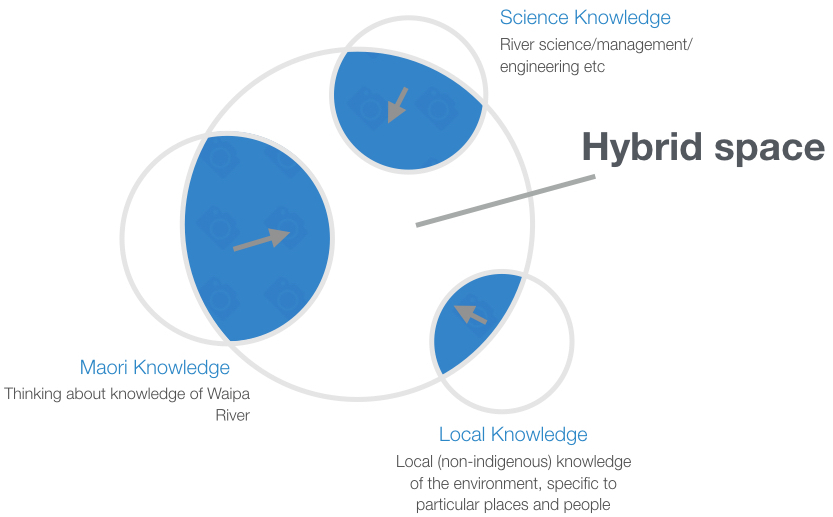
\includegraphics[width=\textwidth]{Fig02.jpeg}}
\captionof{figure}{The different kinds of knowledge creating a hybrid knowledge space in the context of the Waip\={a} River catchment and its management. \label{Fig02}}
\end{minipage}

\begin{multicols}{2}



\section{Way Forward}
\noindent In this paper we have discussed the role of IK in sustainability science and the challenges associated with the inclusion and consideration of IK in scientific discourse in general. We discussed the rationale for considering scientific knowledge and IK as mutually inclusive and useful sources of knowledge in reaching a fuller understanding of sustainability. Our Waip\={a} River case study demonstrates attempts by conventional resource managers and indigenous peoples to utilize different knowledges to inform river management practices. In both cases, we found that the existence of different interpretations of river degradation and identifying possible solutions in a more holistic manner was recognized; however, the extent to which these different knowledges were translated into management plans (and practices) varied.

We argue that there is a need to recognize the influence that environmental determinism and colonialism have in shaping the sustainability research agenda as is the need to pay closer attention
to how research is designed, to what ends, and how communities are framed in research. All too often who is included in ‘society’ and the assessment of desired outcomes is exclusive of indigenous groups and represents mainstream ideologies that have become manifested overtime through visions which in turn have guided modifications of landscapes \citep{r44}. We suggest that scholars need to adopt innovative methodologies that take into account both the historical legacies and present day concerns of indigenous communities about research, which includes confronting the ``lingering imperialism\ldots embedded in self-proclaimed critical methodologies'' \citep{r26}. In our research, we examined the historical records on governance decisions on New Zealand’s landscape modifications \citep{r44}. For the Waip\={a}, we are constructing narratives of river knowledges and practices through historical analyses, interviews with diverse stakeholders, workshops run according to M\={a}ori tradition and cultural practices, and other ethnographic techniques that facilitate the sharing of stories to gain deeper insights into the diverse ideologies and sources of knowledge embedded across time and space.

\textls[-10]{We further propose four key principles that should be applied especially in indigenous-related sustainability research:}

\begin{enumerate}
	\item \textit{Acceptance and advocacy of Indigenous Knowledge systems:} Accepting and adequately representing knowledge systems that do not conform to Western scientific standards. For Indigenous communities, their narratives, oral histories, and cultural practices are essential avenues for knowledge transmission. Hence, approaches that view knowledge systems as contextually-based and located in specific places and times is necessary while also recognizing the broader insights that place-specific IK has.
	\item \textit{Positionality in research:} Critical awareness of how research is shaped by power, relationships, and ethics. This approach views people as collaborators and partners in co- design of research and production of knowledge, rather than merely as informants.
	\item \textit{Co-designing research agenda:} Research agenda needs to be co-designed by Indigenous communities and fit with their priorities.
	\item \textls[15]{\textit{Two-way knowledge sharing:} Since academic research is about searching for `new' knowledge or `new' ways of thinking, researchers rarely consider sharing their research. Sharing knowledge needs to be an ongoing and two-way process. Giving indigenous communities access to all copies of research documents and engaging them in the analysis process will ensure that the results are participatory and representative.}
\end{enumerate}

\textls[10]{We encourage approaches that are explicit about the kind of knowledge each stakeholder group holds as most `valid' to guide the development of solutions to achieving sustainability. In our opinion, such an approach enables a deeper understanding of the diversity of perceptions needed for more holistic approaches to sustainability. This is, however, not always straight forward particularly when ideas embedded in IK and/or policy discourse conflict with researchers' own ideas and values. IK is not a homogeneous body of knowledge and claims of the need to promote a particular traditional practice and way of being can be contested within a cultural group. To respect the diversity found within IK, we as researchers must work with different segments of the communities (e.g. women, younger people, people with disabilities), to ensure appropriate protocols concerning the sharing and representation of IK are accepted across the group.}

In such cases a normative and ethical challenge emerges that requires unpacking how researchers and the groups we work with conceptualize `sustainability', what expectations we share and do not share in terms of how sustainability could be achieved, and what goals and values are ultimately driving these aspirations. While this necessitates the integration of different knowledge systems \citep{r45} and finding ways to accommodate spiritual, material and technical views embedded in natural resource management, it also calls for closer introspection of our own biases, values, and preferences. Creating such diverse yet shared visions of sustainability \citep{r46} can lead to richer and more inclusive ways to tackle solutions.

\end{multicols}
%\clearpage

\vspace{\baselineskip}

\begin{multicols}{2}
\renewcommand*{\refname}{\normalsize{References and Notes}}

\begin{footnotesize}
\bibliographystyle{vancouver_Librello}
\bibliography{274-Biblio}
\end{footnotesize}

\end{multicols}

\end{document}







\vspace{\baselineskip}

\noindent
\begin{minipage}{\columnwidth}
\centering
\resizebox{\columnwidth}{!}
{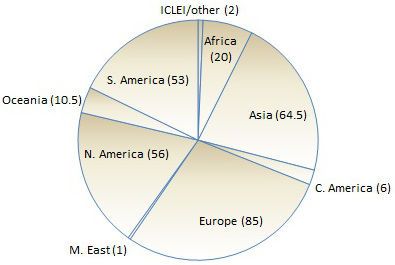
\includegraphics[width=\textwidth]{Fig01.jpg}}
\captionof{figure}{Community gardens in the north of Lisbon (Portugal). \label{Fig01}}
\end{minipage}




\end{multicols}
\vspace{\baselineskip}

\setlength{\tabcolsep}{3pt}
\noindent
\begin{footnotesize}
\begin{minipage}{\columnwidth}\centering
\captionof{table}{Results of a General Linear Model for the proportion of agricultural land under organic farming in French Departments (2008) as a function of plant biodiversity, landscape connectivity, proportion of Natura 2000 protected areas, latitude, longitude, altitude, human population size and department area. The number of data points is 95, the adjusted R$^2$ of the model 0.50, and the intercept 1.457 (s.e. = 2.074).}
\label{Tab01}
\begin{tabular}{lrrrrrrrr}
\toprule
 & N of plant taxa & Landscape connectivity & \% Natura 2000 & Latitude & Longitude & Altitude & Human population & Area \\
\midrule
parameter estimate & 0.264 & 0.047 & 0.113 & -0.084 & 0.003 & 0.038 & 0.056 & 0.327 \\
s.e. & 0.486 & 0.101 & 0.09 & 0.024 & 0.017 & 0.172 & 0.132 & 0.139 \\
\textit{P}-value & 0.59 & 0.64 & 0.21 &\textbf{ \textless0.001} & 0.87 & 0.82 & 0.67 & \textbf{0.02}\\
\bottomrule
\end{tabular}
\end{minipage}

\end{footnotesize}

\vspace{\baselineskip}
\begin{multicols}{2}


\begin{enumerate}[label=\alph*)]
\item
\end{enumerate}